\chapter{Künstliche Neuronale Netze}
Das mathematische Modell von künstlichen neuronalen Netzen wurde von McCulloch und Pitts im Jahre 1943 erfunden \cite{mcculloch1943logical}.
Dieses Modell ist eine Abstraktion des biologischen Neuronen als logischer Mechanismus.
\newline
\newline
Das Nervensystem besteht aus einem Netz von Neuronen, die miteinander verbunden sind und über elektrische Impulse miteinander interagieren \cite{rosenblatt1961principles}.
Man unterscheided beim biologischen Neuronen zwischen \textit{Afferent}-Neuronen, \textit{Efferent}-Neuronen und \textit{Inter}-Neuronen.
Afferent-Neuronen nehmen elektrische Signale von Organen entgegen und können als \textit{Input} interpretiert werden.
Efferent-Neuronen geben elektrische Signale an \textit{Effektorzellen} weiter und können als \textit{Output} interpretiert werden.
Inter-Neuronen nehmen elektrische Signale von Afferent-Neuronen oder Inter-Neuronen entgegen und geben sie an Inter-Neuronen oder Efferent-Neuronen weiter.
Wenn der Schwellenwert eines \textit{Dendrite} von einem Neuronen durch ein elektrisches Signal erreicht wurde, wird ein elektrisches Signal über den \textit{Axon} an ein
anderes Neuron oder Effektorzellen übertragen.
\newline
\newline
Diese Charakteristiken werden mathematisch als ein Vergleich von einer gewichtete Summe von eingehenden Signalen mit einem Schwellenwert modelliert \cite{higham2019deep}.
Gleichung \ref{formular:neuron_activation} stellt diesen Zusammenhang dar.
\begin{align}
    \label{formular:neuron_activation}
    y = \sigma(\sum_{i=1}^n\textbf{w}_i\textbf{x}_i + b)
\end{align}
Die Vergleichsoperation ist die \textit{Aktivierungsfunktion} $\sigma: \mathbb{R}\mapsto\mathbb{R}$, die in diesem Fall ist es die Stufenfunktion.
Die Eingabe $\textbf{x}\in\mathbb{R}^n$ wird mit $\textbf{w}\in[0, 1]^n$ gewichtet und der \textit{Bias} $b\in\mathbb{R}$ wird addiert. Der Bias stellt den Schwellenwert dar.
\newline
\newline
Das künstliche neuronale Netz approximiert eine arbiträre Funktion $f^*$. Dazu findet es eine Menge von Parametern $\boldsymbol\theta$, wodurch $f^*(\textbf{x})\approx f(\textbf{x}, \boldsymbol\theta)$
möglichst gut von der Approximationsfunktion $f$ abgebildet wird \cite{bengio2017deep}.
\newline
\newline
Das KNN ist in Schichten organisiert. Analog zu den biologischen Neuron, gibt es eine \textit{Eingabeschicht (engl. Input-Layer)},
\textit{Ausgabeschicht (engl. Output-Layer)} und \textit{verdeckte Schicht (engl. Hidden-Layer)}.
Analog zur Aktivierung eines einzelnen Neuronen, dargestellt in Gleichung \ref{formular:neuron_activation}, stellt
Gleichung \ref{formular:layer_activation} die Aktivierung einer Schicht dar \cite{higham2019deep}.
\begin{align}
    \label{formular:layer_activation}
    \textbf{a}_{l} = \sigma_l(\textbf{z}_l), \hspace{2cm} \textbf{z}_l := \textbf{W}_l\textbf{a}_{l-1} + \textbf{b}_l
\end{align}
Das allgemeine KNN verfügt über $L\in\mathbb{N}$ Schichten. Jede Schicht $l$ verfügt über $n_l\in\mathbb{N}$ Neuronen.
Die Aktivierungsfunktion $\sigma_l:\mathbb{R}^{n_{l}}\mapsto\mathbb{R}^{n_{l}}$ berechnet die Aktivierung mit der gewichteten Summe $\textbf{z}_l$.
Die gewichtete Summe setzt sich zusammen aus der Aktivierung der vorherigen Schicht $\textbf{a}_l$ die mit $W_i\in\mathbb{R}^{n_{l}x{n_{l-1}}}$ gewichtet wird.
Die Schwellenwerte jedes Neuronen werden durch die Biase $\textbf{b}_l\in\mathbb{R}^{n_{l}}$ dargestellt.
Gleichung \ref{formular:general_knn} zeigt, wie das allgemeine KNN mit einer rekursiven Funktion modelliert werden kann.
\begin{align}
    \label{formular:general_knn}
    \textbf{a}_1 := \textbf{x}, \hspace{1cm}
    \textbf{z}_l := \textbf{W}_l\textbf{a}_{l-1} + \textbf{b}_l, \hspace{1cm}
    \textbf{a}_l := \sigma_l(\textbf{z}_l), \hspace{1cm} \textbf{f(x)} := \textbf{a}_L
\end{align}
Diese Arbeit nutzt ausschließelich \textit{Feed Forward neuronale Netzwerke}.
Diese werden durch \textit{dichte Schichten (engl. Dense-Layer)} charakterisiert, d. h. Schichten in denen alle Neuronen
einer Schicht mit allen Neuronen der folgenden Schicht verbunden sind \cite{bengio2017deep}.

\section{Keras}
Keras ist die am meisten genutzte \textit{deep learning} API und wurde in Python geschrieben \cite{kerasDoc}.
Dadurch ist sie kompatibel mit allen gängigen Betriebssystemen.
Ihr Fokus ist eine intuitive und simple API anzubieten, sodass schnelle Iterationen im Entwicklungsprozess möglich sind.
Trotzdem ist sie effizient und skalierbar, um die Kapazitäten großer Rechenverbunde auszunutzen.
\newline
\newline
Keras abstrahiert das ML System \textit{Tensorflow}. Tensorflow implementiert ML Algorithmen, die dem Stand der Forschung entsprechen.
Der Fokus ist auf effizientes Training der Modelle \cite{abadi2016tensorflow} gerichtet.
Dafür nutzt es die Multikernarchitektur von CPUs, GPUs und spezialisierter Hardware, sogenannten TPUs (\textbf{T}ensor \textbf{P}rocessing \textbf{U}nit), aus.
Es wurde als open-source Projekt veröffentlicht und ist weit verbreitet.
\newline
\newline
Keras bietet die in dieser Arbeit benötigten Algorithmen an, weshalb es zum Trainieren von FFNNs verwendet wird.
\section{Training der ML-Modelle}
\label{sec:model_training}
Typischerweise haben weder Entscheidungsbaum basierte Klassifizierer noch FFNNs Rückwärtskanten.
Neuronale Netze mit Rückwärtskanten werden als \textit{rekurrente Netze} (RNN) bezeichnet.
Abbildung \ref{fig:model_idea} zeigt, dass die Rückwärtskante genutzt wird, um das Klassifizierungsergebnis,
also den vorherigen Standort, bei der Feature-Extrahierung zu nutzen.
Das Klassifizierungsergebnis ist aber nicht immer korrekt, wodurch fehlerhafte Features im Zusammenhang
mit dem Klassifizierungsergebnis als Eingabe in das ML-Modell verwendet werden können.
Damit das ML-Modell lernt mit diesem Fehler umzugehen, ist es notwendig, dass das ML-Modell Trainingsbeispiele mit
Features auf Basis eigener Klassifizierungsbeispiele zur Verfügung hat.
\newline
\newline
Abbildung \ref{fig:training_explained} illustriert den Trainingsablauf.
Die simulierten Daten der aufgenommenen Routen sind unterteilt in Partitionen basierend auf deren Zyklusbeschriftung,
damit in jeder Partition alle Standorte vorhanden sind.
Der Zyklus ist ein Umlauf einer Route, bevor sie wiederholt wird.
Insgesamt besteht die Datenmenge aus 20 Zyklen.
Die ersten fünf Zyklen werden zum \glqq Aufwärmen \grqq\ verwendet,
d. h. das ML-Modell wird mit korrekt beschrifteten Daten trainiert, welche es nicht selbst beschriftet hat.
In den folgenden zehn Zyklen werden weitere Partitionen zur Trainingsmenge hinzugefügt, die mit quadratisch steigendem Anteil vom ML-Modell selbst beschriftet sind.
Zunächst werden 50\% der Partition $i$ vom ML-Modell beschriftet, bis beim 13. Zyklus schließlich 100\% beschriftet wird.
Die Elemente aus der Partition, die beschriftet werden sollen, sind zufällig, damit der Klassifizierungsfehler auf allen Teilstücken der Route gelernt werden kann.
\begin{figure}[h!]
    \centering
    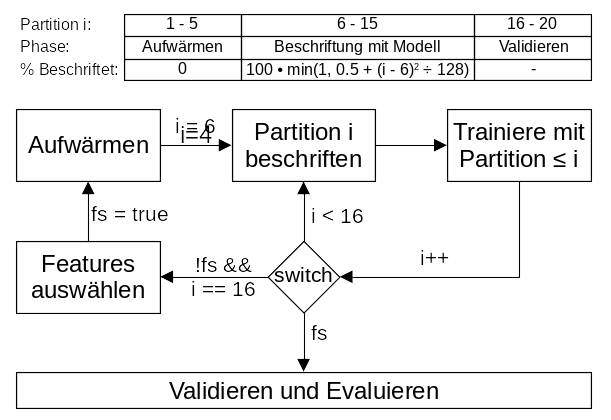
\includegraphics[width=\linewidth]{images/training_explained.png}
    \caption{Der Trainingsablauf des verfolgten Ansatzes.}
    \label{fig:training_explained}
\end{figure}
\newline
\newline
Die erste Trainingsphase ist abgeschlossen, nachdem das ML-Modell mit einer Trainingsmenge von 15 Zyklen trainiert wurde.
Anschließend wird einmalig eine Feature-Auswahl betrieben, in der insignifikante Features aus der Feature-Menge entfernt werden.
Features sind insignifikant, die eine geringe Wichtigkeit aufweisen (Kapitel \ref{sec:eval_feature_importance}).
Dies ermöglicht kleinere ML-Modelle zu verwenden und verringert die Dimensionen des Suchraumes, wodurch das Trainieren erleichtert wird.
Außerdem müssen Modelle individuell für verschiedene Einsatzgebiete trainiert werden, bei denen möglicherweise einige Sensoren bzw. Features nicht genutzt werden.
In Abbildung \ref{fig:training_explained} ist die Feature-Auswahl nur einmalig vorgesehen.
Denkbar wäre aber auch eine iterative Eliminierung der Features oder Optimierung durch ein evolutionären Algorithmus.
Anschließend wird das ML-Modell erneut auf den Partitionen trainiert, bis es validiert und evaluiert werden kann.
\newline
\newline
Die ML-Modelle ohne Rückwärtskante sind deutlich simpler.
Diese müssen nicht in Zyklen trainiert werden, sondern können direkt mit der vollständigen Trainingsmenge trainiert werden,
wodurch das Training deutlich effizienter ist.
\section{Optimierer}
Die Strategie im Optimierungsprozess wird als Optimierer bezeichnet.
Diese Algorithmen steuern, wie die Parameter $\boldsymbol\theta$ aktualisiert werden.
Die Eingabe sind die Kosten der Trainingsdaten.
Üblicherweise wird \textit{ADAM} verwendet.
ADAM ist eine Kombination aus \textit{SGD} (\textbf{S}tochastic \textbf{G}radient \textbf{D}escent) mit Momentum und \textit{RMSprop}.
\newline
\newline
SGD ist eine Approximation von \textit{Gradient Descent} (GD).
GD ist ein iterativer Algorithmus, der den Gradienten in Richtung des Extrema folgt und dementsprechend die Eingabeparameter aktualisiert.
\begin{align}
    \label{formular:gradient_descent}
    x_{k+1} := \begin{cases}
                   x_k - C^{\prime}(x_k)\alpha_k & \text{, wenn } C(x_k - C^{\prime}(x_k)\eta_k) < C(x_k)\\
                   (1 + \alpha_k)x_k & \text{, ansonsten}
    \end{cases}
\end{align}
Gleichung \ref{formular:gradient_descent} illustriert diesen iterativen Prozess für Minimierung im eindimensionalen Fall,
wobei $\eta_k > 0$ eine angemessene \textit{Lernrate} ist, $x$ der Eingabeparameter und $C$ die Kostenfunktion.
Ist die Lernrate zu groß könnte keine Verbesserung beobachtet werden, da das Maxima immer übersprungen wird.
Ist die Lernrate zu klein könnte die Konvergenz sehr langsam sein.
\newline
\newline
Im mehrdimensionalen Fall wird für jede Komponente des Eingabevektors dieser Prozess durchgeführt, sodass für jede Komponente
die Richtung des Extrema verfolgt wird.
Dies impliziert, dass GD sehr aufwendig zu berechnen ist für Eingabevektoren mit hohen Dimensionen.
Gleichung \ref{formular:gd_multi_dim} zeigt die iterative Berechnung im mehrdimensionalen Fall.
\begin{align}
    \label{formular:gd_multi_dim}
    \textbf{x}_{k+1} = \textbf{x}_k - \bigtriangledown C(\textbf{x}_k)\eta_k
\end{align}
Zur Berechnung muss der Gradient des Eingabevektors berechnet werden.
Je größer die Dimension des Eingabevektor ist, desto aufwendiger ist die Berechnung.
\newline
\newline
SGD nimmt an, dass eine Verbesserung wahrscheinlich ist, wenn eine Komponente, bzw. ein \textit{mini-batch} (Teilmenge), des
Eingabevektors in Richtung des Extrema aktualisiert wird.
Aus diesem Grund werden die Parameter aktualisiert, nachdem jeweils nur eine Komponente des Eingabevektors aktualisiert wurde.
Dadurch bedarf das neuronale Netzwerk zur Konvergenz mehr Epochen, muss aber weniger Berechnungen durchführen.
\newline
\newline
(S)GD mit Momentum versucht zu vermeiden, dass lokale Extrema gefunden werden anstatt globale Extrema, indem Momentum aus
vorherigen Gradienten beibehalten wird, um aus lokalen Extrema wieder raus zu finden.
Gleichung \ref{formular:sgd_momentum} zeigt die iterative Berechnung.
\begin{align}
    \label{formular:sgd_momentum}
    \textbf{v}_{-1} = \textbf{0}, \hspace{0.6cm} \textbf{v}_k = \textbf{v}_{k-1}\gamma +
    \bigtriangledown f(\textbf{x}_k), \hspace{0.6cm} \textbf{x}_{k+1} = \textbf{x}_k - \textbf{v}_k\eta
\end{align}
Zur Berechnung wird ein Hilfsvektor $\textbf{v}$ verwendet, welcher das Momentum vergangener Gradienten darstellt.
In jeder Iteration fließt ein Anteil $\gamma$, typischerweise $\gamma=0.9$, von dem Hilfsvektor in die Berechnung der neuen Eingabeparameter ein.
Der Unterschied zum GD (\ref{formular:gd_multi_dim}) ist der Anteil vergangener Gradienten.
\newline
\newline
RMSprop ist eine Variante von \textit{Adagrad}.
Adagrad passt die Lernrate $\eta$ an, denn typischerweise wird zuerst eine hohe Lernrate benötigt und je näher sich dem Extrema angenähert wird,
sollte diese Lernrate sinken.
Gleichung \ref{formular:adagrad} zeigt, wie sich iterativ die Lernrate antiproportional
zur kummulierten Norm der Gradienten der Kostenfunktion verringert.
Dabei wird für $\epsilon$ eine kleine Zahl gewählt, um Teilen durch 0 zu vermeiden aber keinen signifikanten Einfluss auf die Berechnung zu haben.
\begin{align}
    \label{formular:adagrad}
    \textbf{g}_k = \bigtriangledown C_{j_k}(\textbf{x}_k), \hspace{0.6cm}
    \textbf{w}_k = \textbf{w}_{k-1} + \textbf{g}_k^2, \hspace{0.6cm}
    \textbf{x}_{k+1} = \textbf{x}_k - \textbf{g}_k \circ \frac{\eta}{\sqrt{\textbf{w}_k + \epsilon}}
\end{align}
Das Problem an Adagrad ist, dass die Lernrate zu schnell gegen 0 konvergieren kann, wodurch das Zielextrema nicht erreicht wird.
RMSprop (\ref{formular:rmsprop}) löst dieses Problem, indem in jeder Iteration ein Zerfallsfaktor $\gamma < 1$ auf den Hilfsvektor $\textbf{w}$ angewendet wird
und Anteilweise das Hadamard-Produkt des Gradienten der Kostenfunktion addiert wird.
\begin{align}
    \label{formular:rmsprop}
    \textbf{w}_{-1} = \textbf{0}, \hspace{0.6cm}
    \textbf{g}_k = \bigtriangledown C_{j_k}(\textbf{x}_k), \hspace{2cm} \nonumber\\
    \textbf{w}_k = \textbf{w}_{k-1}\gamma + \textbf{g}_k^2 (1-\gamma), \hspace{0.6cm}
    \textbf{x}_{k+1} = \textbf{x}_k - \textbf{g}_k \circ \frac{\eta}{\sqrt{\textbf{w}_k + \epsilon}}
\end{align}
Gleichung \ref{formular:adam} zeigt, wie Adam RMSprop und SGD mit Momentum vereint, wobei $\gamma_1 < \gamma_2 < 1$.
Adam nutzt zwei Hilfsvektoren $\textbf{v}$ und $\textbf{w}$, die mit einer Zerfallsrate wachsen und beim Lernen
sowohl Momentum nutzt, um lokale Extrema zu überbrücken, und passt die Lernrate im Laufe des Trainingsprozesses an.
\begin{align}
    \label{formular:adam}
    \textbf{v}_{-1} = \textbf{w}_{-1} = \textbf{0}, \hspace{3.5cm} \nonumber\\
    \textbf{g}_k = \bigtriangledown C_{j_k}(\textbf{x}_k), \hspace{0.6cm}
    \textbf{v}_k = \textbf{v}_{k-1}\gamma_1 + \textbf{g}_k (1-\gamma_1), \hspace{1cm} \nonumber\\
    \textbf{w}_k = \textbf{w}_{k-1}\gamma_2 + \textbf{g}_k^2 (1-\gamma_2), \hspace{0.6cm}
    \textbf{x}_{k+1} = \textbf{x}_k - \textbf{v}_k \circ \frac{\eta}{\sqrt{\textbf{w}_k + \epsilon}}
\end{align}
\section{Aktivierungsfunktionen}
Die Aktivierungsfunktion entscheided ob ein Neuron aktiviert wird oder nicht \cite{nwankpa2018activation}.
Sie können entweder linear oder nicht-linear sein.
Es ist aber nötig nicht-lineare Funktionen zu verwenden, damit jede kontinuierliche Funktion approximiert werden kann \cite{apicella2021survey}.
Sie unterscheiden sich in ihren Eigenschaften und Berechnungskosten, was eine besondere Rolle für Mikrocontroller spielt.
\newline
\newline
In der frühen Geschichte der neuronalen Netzwerke wurde die \textit{Sigmoid}-Funktion (\ref{formular:af_sigmoid}) viel verwendet, da sie asymptotisch begrenzt,
kontinuierlich und nicht-linear ist \cite{apicella2021survey}.
Oft wird sie heute in der Ausgabeschicht für binäre Klassifizierungsprobleme eingesetzt \cite{nwankpa2018activation}.
Allerdings ist sie für tiefe neuronale Netzwerke ungeeignet, da der Gradient zwischen 0 und 0.25 ist und dadurch im
Backpropagation-Prozess bereits nach wenigen Schichten gegen 0 geht.
Die \textit{SoftMax}-Funktion (\ref{formular:af_softmax}) oder normalisierte Exponentialfunktion berechnet für einen Eingabevektor eine Wahrscheinlichkeitsverteilung.
Die Einträge dieser Verteilung können für die Wahrscheinlichkeiten der einzelnen Klassen eines multivariat Klassifizierungsproblem interpretiert werden.
\begin{align}
    \label{formular:af_sigmoid}
    \text{sigmoid}(x) = \frac{1}{1 + e^{-x}}
\end{align}
\begin{align}
    \label{formular:af_softmax}
    \text{softmax}(x_i) = \frac{e^{x_i}}{\sum_j e^{x_j}}
\end{align}
\subfigbox{
\subfigure[Sigmoid/SoftMax]{\label{subfig:af_sigmoid}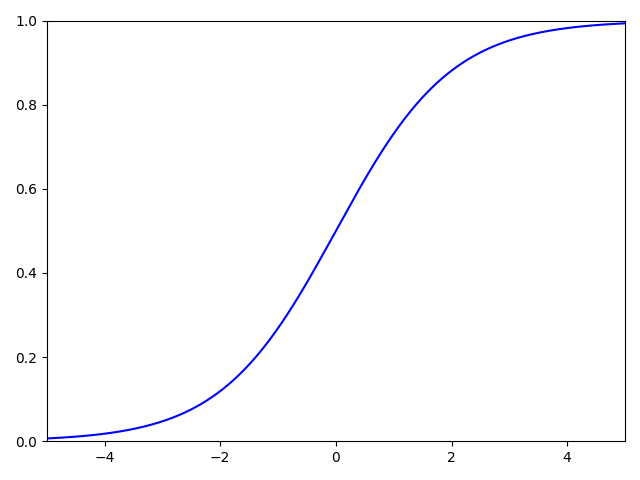
\includegraphics[width=0.495\linewidth]{images/activation_function_heaviside.png}}\hfill%
\subfigure[ReLU Varianten]{\label{subfig:af_relu}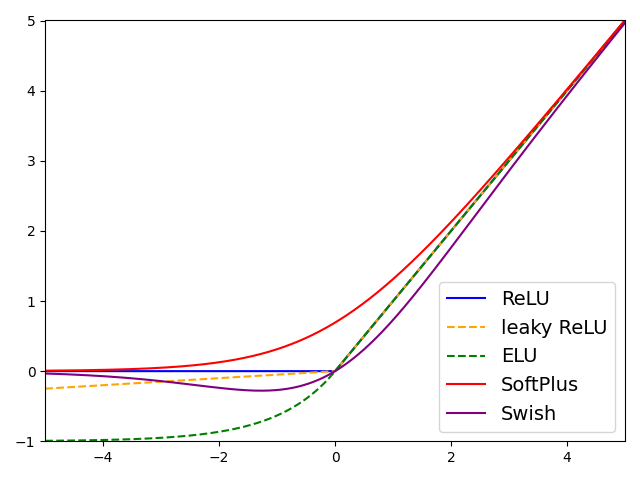
\includegraphics[width=0.495\linewidth]{images/activation_function_relu_varianten.png}}
}{Verschiedene Aktivierungsfunktionen.}{fig:activation_functions}
\newline
\newline
Zur \textit{ReLU}-Familie \cite{apicella2021survey} gehört die ReLU-Funktion \cite{glorot2011deep, konda2014zero, elfwing2018sigmoid, alcaide2018swish} und
ihre Varianten \cite{maas2013rectifier}, sowie die \textit{SoftPlus}- \cite{dugas2001incorporating} und \textit{Swish}-Funktion \cite{ramachandran2017searching}.
ReLU (\ref{formular:af_relu}) steht für \glqq\textit{rectified linear function}\grqq\ und wird häufig in modernen neuronalen Netzwerken verwendet \cite{apicella2021survey}.
Sie ist nicht differenzierbar bei 0 und die Ableitung für negative Eingaben ist 0.
Dies kann zu \textit{sterbenden Neuronen (engl. dying neurons)} führen, da der Bias so negativ wird, sodass das Neuron nicht mehr aktiviert wird.
Zudem ist der Trainingsprozess verlangsamt, wenn der Gradient konstant 0 ist.
Dafür ist die Ableitung der Funktion ansonsten 1, was den Backpropagation-Prozess vereinfacht, da der Gradient neutral zur Aktivierungsfunktion ist.
\begin{align}
    \label{formular:af_relu}
    \text{ReLU}(x) = \max(x, 0)
\end{align}
Varianten sind beispielsweise \textit{leaky ReLU} \cite{maas2013rectifier} (\ref{formular:af_leaky_relu}) und \textit{ELU (exponential linear unit)} (\ref{formular:af_elu})
\cite{clevert2015fast}, welche versuchen die Defizite des konstanten 0 Gradienten zu lösen, indem der negative Teil der Funktion nicht 0 ist.
\begin{align}
    \label{formular:af_leaky_relu}
    \text{leaky\_ReLU}_{\alpha}(x) = \begin{cases}
                               x & \text{, wenn } x \geq 0\\
                               \alpha x & \text{, ansonsten } (\alpha\in \mathbb{R}_{0}^{+})
    \end{cases}
\end{align}
\begin{align}
    \label{formular:af_elu}
    \text{ELU}_{\alpha}(x) = \begin{cases}
                                 x & \text{, wenn } x \geq 0\\
                                 \alpha(e^{x} - 1) & \text{, ansonsten } (\alpha\in \mathbb{R}_{0}^{+})
    \end{cases}
\end{align}
\textit{SoftPlus} (\ref{formular:af_softplus}) ist analytisch, dafür im Vergleich zu ReLU aufwendiger zu berechnen ist\cite{apicella2021survey}.
\begin{align}
    \label{formular:af_softplus}
    \text{softplus}(x_i) = \ln(e^x + 1)
\end{align}
Eine weitere Variante ist \textit{Swish} \cite{ramachandran2017searching} (\ref{formular:af_swish}).
Sie ist analytisch aber nicht monoton.
Im Vergleich zu ReLU ist sie aufwendig zu berechnen.
Ihre Autoren behaupten aber, dass dadurch bessere Ergebnisse erzielt werden können, ohne andere Parameter zu ändern.
\begin{align}
    \label{formular:af_swish}
    \text{swish}(x_i) = \frac{xe^x}{e^x + 1}
\end{align}
\section{Ressourcenbedarf auf dem Mikrocontroller}
\label{sec:dt_resource_usage}
Zukünftig soll das Modell auf einem Mikrocontroller ausgeführt werden \cite{antragForschungsprojekt}.
Mikrocontroller sind stark limitiert in ihrer Rechenleistung, Speicherkapazität, RAM und werden oft zudem mit einer Batterie betrieben.
Aus diesem Grund ist der Energieverbrauch zu minimieren und das Modell muss innerhalb dieser Limitierungen operieren können.

\newpage
\subsection{Ausführungszeit und Energieverbrauch}
\label{sub_sec:dt_ru_execution_time}
Der Energieverbrauch korreliert mit der Ausführungszeit.
Je länger die CPU ausgeschaltet ist, desto weniger Energie wird verbraucht.
Kurze Ausführungszeiträume vergrößern den Zeitraum, in dem die CPU ausgeschaltet sein kann.
Die Ausführungszeit ist die Zeit die benötigt wird, um alle Instruktionen auszuführen \cite{dymelThesis}.
Jede Instruktion bedarf eine bestimmte Anzahl an CPU-Zyklen.
Die Zeit pro Zyklus ist abhängig von der Taktrate der CPU.
\newline
\newline
Die Ausführungszeit eines Entscheidungswaldes setzt sich zusammen aus der Zeit für die Feature-Extrahierung, der Evaluierung aller im Ensemble enthaltenen Entscheidungsbäume
und der Aggregierungsfunktion.
Im schlimmsten Fall muss die gesamte Höhe eines Entscheidungsbaumes traversiert werden, um das Ergebnis zu bestimmen. Aus diesem Grund skaliert die Ausführungszeit mit der
traversierten Höhe jedes Baumes.
\newline
\newline
Um die Instruktionen zu minimieren sollten Datentypen verwendet werden, die von der CPU mit höchstens einem Wort dargestellt werden können.
Eine 8-Bit CPU würde zum Laden in Register eines 32-Bit Datentypen vier mal so viele Instruktionen benötigen wie bei einem 8-Bit Datentypen.
Außerdem sollten Operationen verwendet werden, die durch native Hardware-Operationen abgebildet werden können.
Ist dem nicht so, muss diese Operation durch Software ersetzt werden.
Dies erfordert mehr Zyklen als eine native Operation in Hardware.
\newline
\newline
Zu Beachten bei der Minimierung ist, dass Instruktionen unterschiedlich viele Zyklen benötigen und Funktionsaufrufe Overhead erzeugen.
Ein Beispiel dafür ist die Optimierung \textit{Function Inlining} \cite{leupers1999function}.
Der Aufruf von Funktionen kann einen hohen Overhead durch den Kontextwechsel erzeugen.
Aus diesem Grund verringert diese Optimierung die Ausführungszeit, erhöht aber die die Programmgröße signifikant.
Im Umkehrschluss könnten durch die Verwendung von Funktionen der nutzen des Programmspeichers verringert werden, Ausführungszeit und Energieverbrauch aber erhöht werden.

\newpage
\subsection{Programmgröße}
\label{sub_sec:dt_ru_programm_size}
Die Programmgröße ist die Gesamtheit aller Instruktionen die für das Programm benötigt werden \cite{dymelThesis}.
Dabei ist der Anteil für die Entscheidungswälder integral und der Anteil für die perifären Funktionalitäten zu vernachlässigen.
Die Programmgröße, die für einen Entscheidungswald benötigt wird, skaliert mit der Waldgröße und Höhe der einzelnen Entscheidungsbäume.
\newline
\newline
Die Höhe des Entscheidungsbaumes ist die Verzweigungstiefe der verschachtelten Tests.
Jeder Test ist ein Vergleich mit einem Schwellenwert.
Die Programmgröße für einen Vergleich setzt sich zusammen aus den Operationen um die Operanden in die Register zu laden
und die Instruktion um den Vergleich durchzuführen, sowie Abzweiginstruktionen. Wie in Kapitel \ref{sub_sec:dt_ru_execution_time}
sind Instruktionen durch einen passenden Datentypen zu vermeiden.
\newline
\newline
Ein weiterer Faktor sind die Instruktionen, die zur Rückgabe des Klassifizierungsergebnis benötigt werden.
In Kapitel \ref{sec:dt_ensemble_methods} wurden verschiedene Möglichkeiten der Rückgabe diskutiert, die relevant bei dem Aggregierungsprozess eines Ensembles ist.
Einerseits kann die Rückgabe eine Wahrscheinlichkeitsverteilung sein und andererseits eine diskrete Klasse.
Bei $m$ möglichen Klassen würde die erste Variante $m$-mal so viele Instruktion benötigen, wie die zweite Variante, da der Rückgabevektor zuvor mit der Wahrscheinlichkeitsverteilung gefüllt werden muss.
In der Praxis werden aber weniger Instruktion benötigt, da es eine große Überschneidung der Wahrscheinlichkeitsverteilungen gibt, die zurück gegeben werden.
Die Instruktionen, um den Rückgabevektor zu befüllen, können durch \textit{Basic Blocks}, d. h. beschriftete Instruktionsblöcke, geschickt recycled werden.
Zudem können Zuweisungen ausgelassen werden, die die Wahrscheinlichkeit 0 zuweisen, da der Vektor mit Nullen initialisiert wird.
Dennoch werden signifikant mehr Instruktionen benötigt als bei der diskreten Variante.
Aus diesem Grund wurde ein hybrider Ansatz vorgeschlagen, der im Falle eines eindeutigen Ergebnisses mit einer Toleranz von $\epsilon\in [0, 1]$ die diskrete Klasse statt der Wahrscheinlichkeitsverteilung zurück gibt.